\documentclass{article}
\usepackage{graphicx, amssymb, amsmath}

\begin{document}

\title{Extended Gravitational Lens: Thin Approximation Inadequacy}

\maketitle

\section{-}

Let $O$, $S$ and $L$ to denote the Observer, Source and Lens respectively. $P$ denotes some arbitrary point on the ray of light. The lens is assumed to be spherically symmetric, the Schwarzschild orbital equation for massless particles (the lensing equation)is then:
\begin{equation}
    \label{eq1}
    \frac{d^2u}{d\theta^2}+u=3r_gu^2
\end{equation}
where $u\equiv1/r$, the radius $r\equiv \overline{LP}$, and $\theta\equiv \angle SLP$.
The gravitational radius  
\begin{equation}
    \label{eq2}
    r_g(r) \equiv \frac{M(r)G}{c^2}
\end{equation}
is a function of $r$, here $c$ is the speed of light and $M(r)$ the lens mass enclosed by a sphere of radius $r$. We define the impact point $B$ as a point on the ray where $\theta=\pi/2$. The impact parameter is then $b \equiv \overline{LB}=u(\pi/2)^{-1}$. The angle between $\vec{SL}$ and the ray tangent is called the "ray angle":
\begin{equation}
    \label{eq3}
    \alpha \equiv \arctan \left( \frac{-u^{-1}u'\sin \theta + \cos \theta}{-u^{-1}u'\cos \theta - \sin \theta} \right) \;.
\end{equation}
$\alpha(0)$ and $\alpha(\theta_O)$ are the incoming and outgoing angles respectively, $\theta_O\equiv \angle SLO$.

For thin lens approximation light is assumed to travel in a straight line from $S$ to $B$, where it is deflected by an angle $\gamma=4r_g/b$, the mass used to calculate $r_g$ is the lens projected mass in a circle of radius $b$.

Calculating the time of travel is done as follows:
\begin{equation}
    \label{eq4}
    \Delta t_{ray} = \int_{Ray} \frac{dp}{c} \left( 1- \frac{r_g}{r(p)}\right)^{-\frac{1}{2}} 
\end{equation}
the square root term is the regular gravitational time dilation.

\section{The harmonic solution to the lensing equation}

We are interested in solving the lensing equation (eq. \ref{eq1}) inside an isothermal sphere sharply truncated at $R$. The total mass is $M_0$ and the enclosed mass $M(r)=M_0r/R$. Plugging this into the lens equation (eq. \ref{eq1}) gives:
\begin{equation}
    \label{eq5}
    \frac{d^2u}{d\theta^2}=\left( \frac{3M_0G}{Rc^2} -1 \right) u \;.
\end{equation}
This is the equation of an harmonic oscillator with $m=1$ and
\begin{equation}
    \label{eq6}
    k=\left( 1-\frac{3M_0G}{Rc^2} \right) u \;.
\end{equation}
The general solution is $u=A\cos \left( \omega \theta+\phi \right)$ with $\omega=\sqrt{k/m}$ i.e.
\begin{equation}
    \label{eq7}
    u= A \cos \left( \theta\sqrt{1-\frac{3M_0G}{Rc^2}} +\phi \right)
\end{equation}
where $\phi$ and $A$ are decided by the boundary conditions. We are interested in a symmetric configuration around the lens, the hence the $\cos$ term has to be maximal at $\theta=\pi/2$ 
\begin{equation}
    \label{eq8}
    \phi = -\frac{\pi}{2}\sqrt{1-\frac{3M_0G}{Rc^2}}
\end{equation}
At the same point where the $\cos$ is maximal ($\theta=\pi/2$) we define the impact point, giving $A=1/b$. The symmetric solution is then 
\begin{equation}
    \label{eq9}
    u= \frac{1}{b} \cos \left( \sqrt{1-\frac{3M_0G}{Rc^2}} \left( \theta-\frac{\pi}{2}\right) \right)\;.
\end{equation}
This solution is uniquely defined by the total halo mass $M_0$, its radius $R$ and the impact parameter $b$.

\section{One specific example}
We compare three solutions to a lensing configuration: analytical (harmonic), numerical, and thin approximation. The configuration is cosmologically driven, the lens total mass $M_0=2\times 10^{12} M_s/h$, the lens radius $R=200 Kpc/h$ and the impact parameter $b=4 Kpc/h$. We solve the analytic solution inside the halo, and fit to it a numerical solution to the general lensing equation. The numerical solution fits the analytical one very good, it is defined outside of the halo and it preserves symmetry. We put a source at $rs = u_{num}(0)^{-1}=3.5477249 Gpc/h$ and run a thin lens ray with the same incoming angle as the numerical one. To calculate the projected mass inside the cylinder or radius $b$ we first calculate the projected density of the lens:
\begin{align}
    \rho &= \frac{   {\rm d}M(r)   }{   {\rm d}r   } \frac{1}{4\pi r^2}\\
    &= \frac{M_0}{4\pi Rr^2}\\
    \Psi&=2\int_0^{\sqrt{R^2-r_p^2}} \rho(\sqrt{r_p^2+z^2}) {\rm d}z \\
    &=\frac{M_0}{2\pi R} \int_0^{\sqrt{R^2-r_p^2}} \frac{{\rm d} z}{r_p^2+z^2} \\
    &=\left[ \frac{M_0}{2\pi R r_p} \arctan \frac{z}{r_p} \right] _0^{\sqrt{R^2-r_p^2}}\\
    &=\frac{M_0}{2\pi R r_p}\arctan \sqrt{\frac{R^2}{r_p^2}-1}
\end{align}
where $r_p\equiv \sqrt{x^2+y^2}$ is a projected radius. The mass inside a cylinder of radius $b$ is then a simple 1D integral of the cylindrical shells:
\begin{align}
    M_{projected}(b) &= \int_0^b 2\pi r_p \Psi(r_p) {\rm d} r_p \\
    &= \frac{M_0}{R} \int_0^b \arctan \left( \sqrt{\frac{R^2}{r_p^2}-1} \right) {\rm d} r_p\;.
\end{align}
This has an analytical solution, but we just integrate this with a simple 1D quadrature. For our configuration, $M_{projected}(4 Kpc/h) = 6.24318\times 10^{10} M_s/h$ (this is 56\% higher than the enclosed mass in a similar radius sphere). We run the thin ray with the above configuration and we find that it diverges significantly from the numerical and analytical solutions, see figures below. To test that our solution for the thin ray is good, we compare it to the numerical solution in a different scenarion in which the rays miss the halo, see last figure in this document (the source is on the left). This configuration consists of a black hole lens of mass $2\times 10^{12}M_s/h$, a source at a distance of $3.3 Gpc/h$ and an impact parameter $b=20 Kpc/h$ (yea, this is less cosmologically driven but it should get the idea across, that thin lens matches our numerics for non extended configurations) 

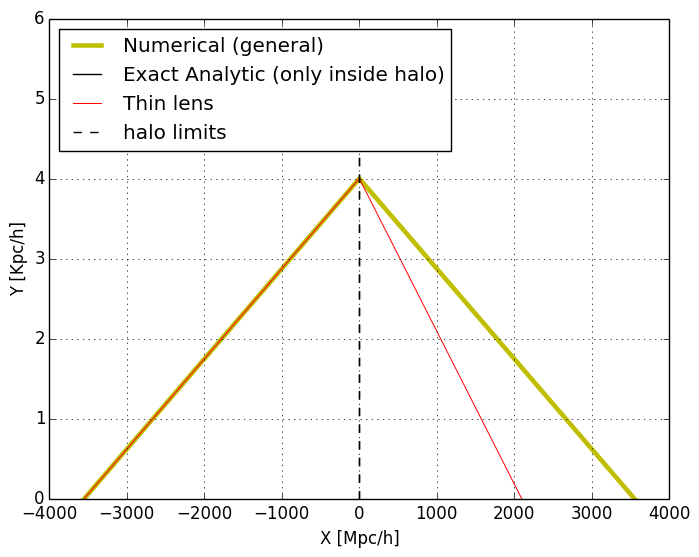
\includegraphics[width=300pt]{zoom_1.png}

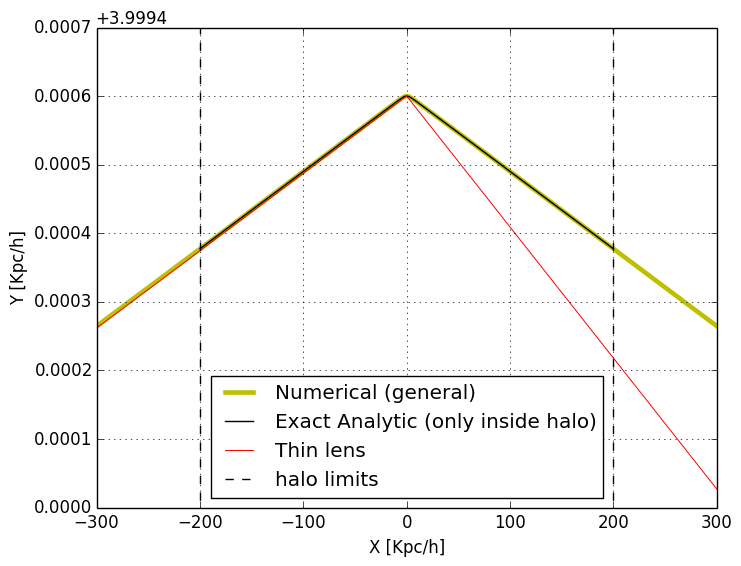
\includegraphics[width=300pt]{zoom_2.png}

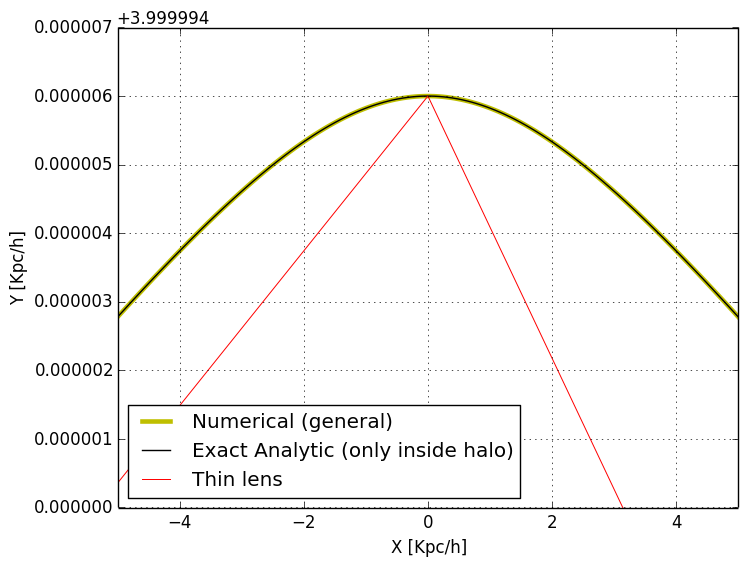
\includegraphics[width=300pt]{zoom_3.png}

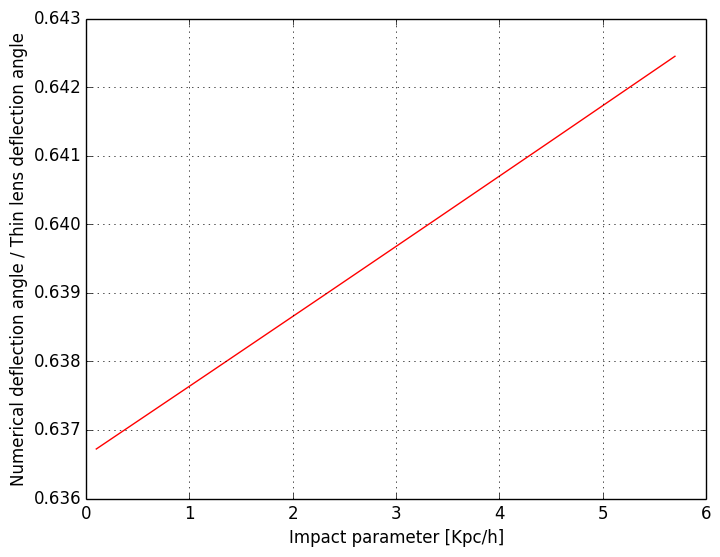
\includegraphics[width=300pt]{u1.png}

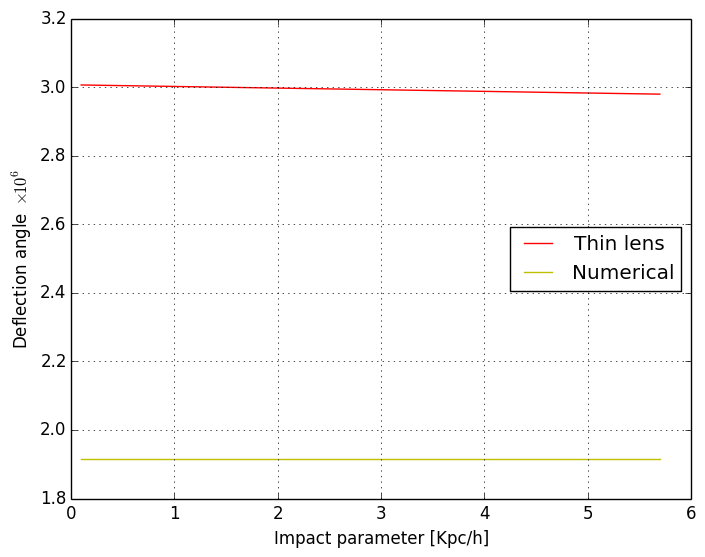
\includegraphics[width=300pt]{u2.png} 

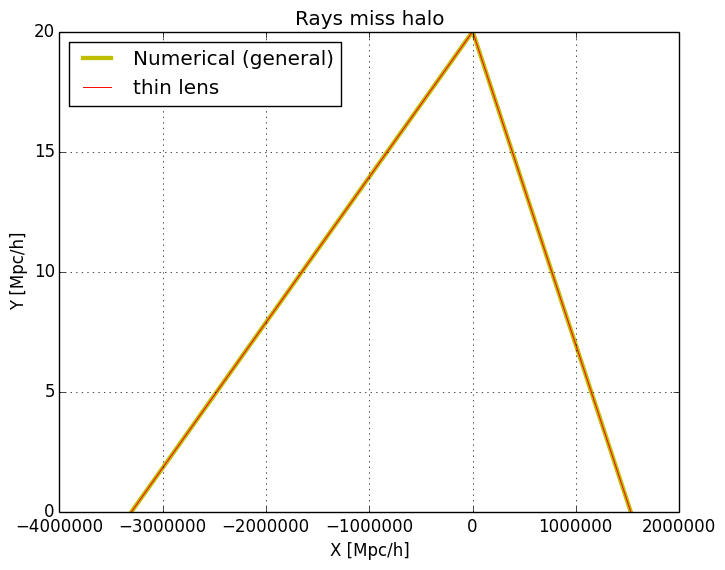
\includegraphics[width=300pt]{missing_the_lens.png} 

\end{document}
